\scanpage{15}
\begingroup
\makeatletter
\tagsleft@true
\makeatother
\uline{\deleted{\unsure{I|V}}\unsure{Version} I}

Soient $X$ un espace topologique, $(\deleted{\unsure{\Sigma|S}}E_i)_{i\in I}$ un ens. de parties \inserted{\unsure{fermés|fermées}} de $X$ (noté indiciellement), telles que l'on ait
% slanted
\reversemarginpar
\margin{$\nearrow$ On suppose de plus que pour \unsure{tte|toute|tt} comp. \unsure{conn.|connex.} $\Sigma_{\unsure{i}}$ de $X\setminus E_i$, on ait $\overline{\Sigma}_i\cap E_i\ne\varnothing$ i.e. $\overline{\Sigma}_i\ne\Sigma_i$ i.e. $\Sigma_i$ \unsure{non} fermé dans $X$ (ce qui est le cas si $X$ est connexe)}
\normalmarginpar
\[
 \forall i\in I,\quad \operatorname{Card}\pi_0(X\setminus\deleted{\Sigma}E_i)=2
 \tag*{(a)}
\]
\margin{\uline{NB} les comp. conn. $\Sigma_i^+,\Sigma_i^{\unsure{+|-|\ast}}$ de $X\setminus\unsure{\Sigma|E}_i$ sont ouvertes dans $X$}
\[
 \begin{aligned}
 &\forall(i,j)\in I\times I,\ i\ne j,\quad \deleted{\Sigma}E_j\ \text{est contenu dans l'une}\\
 &\text{des deux composantes connexes de }X\setminus\deleted{\unsure{\Sigma}}E_i.
 \end{aligned}
 \tag*{(b)}
\]

NB Cette condition (b) est vérifiée \unsure{automatiquement} les $\deleted{\Sigma}E_i$ $(i\in I)$ sont connexes, dès lors que les $E_i$ sont supposés disjoints mutuellement

On se propose d'étudier le ``découpage'' de $X$ par la famille $(E_i)$.

\uline{Cas $\operatorname{Card}\deleted{\unsure{(\mathrm{de})}}(I)\deleted{\unsure{\leq|=}}=2$}

Soit $\Sigma_i^+$ la comp. conn. de $X\setminus E_i$ qui ne contient pas $E_j$ $(j\ne i)$, alors on a (si $I=\{1,2\}$)
\figure{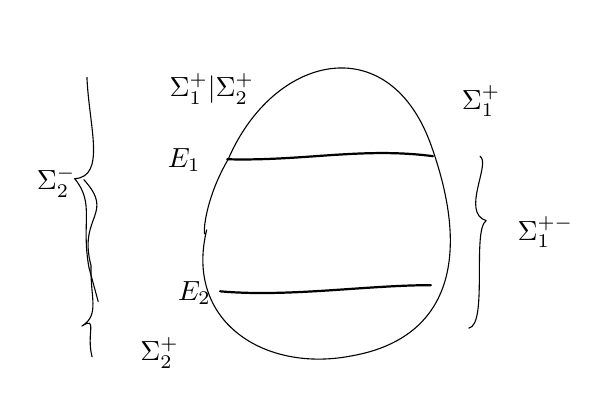
\begin{tikzpicture}[x=.013cm,y=-.013cm,line cap=round,line join=round]
\draw (182,89) .. controls (226,-13) and (337,-39) .. (379,72)
 .. controls (423,192) and (393,265) .. (303,281)
 .. controls (217,298) and (139,247) .. (161,158)
 .. controls (157,176) and (155,135) .. (182,89);
\draw[line width=.8pt] (181,89) .. controls (256,91) and (313,77) .. (382,86)
 (174,218) .. controls (240,224) and (317,212) .. (380,212);
\draw (44,9) .. controls (46,57) and (63,106) .. (32,108)
 .. controls (52,132) and (38,151) .. (46,195) -- (55,228);
\draw (41,109) .. controls (72,143) and (35,144) .. (48,193)
 .. controls (47,224) and (57,241) .. (39,252) .. controls (55,242) and (43,259) .. (49,282);
\draw (428,86) .. controls (439,93) and (409,141) .. (434,149)
 .. controls (420,158) and (436,251) .. (417,254);
\node at (166,20) {$\deleted{\unsure{\Sigma_1^+|\Sigma_2^+}}$};
\node at (139,90) {$E_1$}; \node at (149,220) {$E_2$};
\node at (429,32) {$\Sigma_1^+$}; \node at (492,160) {$\Sigma_1^{\deleted{\unsure{+}}\unsure{-}}$};
\node at (14,111) {$\Sigma_2^-$}; \node at (115,278) {$\Sigma_2^+$};
\end{tikzpicture}}
\[
 \Sigma_1^+\cap\Sigma_2^+=\varnothing
 \tag*{(1)}
\]
ce qui \deleted{résulte de} \unsure{équivaut} à
\[
 \begin{aligned}
 &\deleted{\Sigma_1^-\supset\Sigma_2^+}\\
 &\deleted{\Sigma_2^-\supset\Sigma_1^+}\qquad \Sigma_1^+\subset\Sigma_2^-\cup E_2,\quad\text{et}
 \end{aligned}
\]
\deleted{\unsure{car si}} \deleted{Si on avait} comme $\Sigma_1^+\cap E_2=\varnothing$, cela équivaut aussi à
\[
 \Sigma_1^+\subset\Sigma_2^-
 \tag*{(2)}
\]
\unsure{et} symétriquement, à
\[
 \Sigma_2^+\subset\Sigma_1^-
 \tag*{$(2')$}
\]

Comme \deleted{\unsure{vois. ouvert}} $\Sigma_2^-\supset E_1$, \deleted{il contient les} \inserted{i.e. $\Sigma_2^-$ est un \uline{vois.} ouvert de $E_1$,} on a
% slanted
\reversemarginpar
\margin{$\overline{\Sigma_1^+}\cap E_1\ne\varnothing$ i.e. $\overline{\Sigma_1^+}\ne\Sigma_1^+$ \unsure{à signaler|à sign.ler} avant}
\normalmarginpar
\[
 \Sigma_2^-\cap\Sigma_1^+\ne\varnothing
\]
Car $\underline{\overline{\Sigma_1^+}\cap E_1}\ne\varnothing$ (sinon \inserted{l'ouvert} $\Sigma_1^+$ serait \inserted{\unsure{un|une}} fermé dans $X$, \unsure{donc|puis} \deleted{\unsure{\Sigma_1^+\text{ serait}}} $X$ serait disconnexe),
\endgroup
% archive sheet number: 14
